\documentclass[a5paper,12pt]{article}
\usepackage{../../../style}


\newcommand{\montitre}{Synchronisation }


\begin{document}

\fiche{Multiprogrammation}
\titre{Ressource :} 
	\begin{itemize}
		\item wiki-du-lama
		\item Systèmes d'exploitation (A. Tanenbaum) chap 2 et 6
	\end{itemize}

\titre{Définition :} La multiprogrammation, c'est exécuter simultanément plusieurs programmes sur une même machine, un même CPU, en basculant rapidement de l'un à l'autre, créant une impression de simultanéité. \\

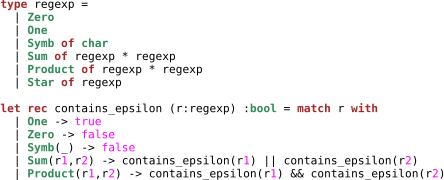
\includegraphics[width=200px]{fig1.pdf}

\begin{tabular}{cccc}
	 & Proc1 & Proc2 & Proc3 \\ \hline
	R0 & $\ldots$ & $\ldots$ & $\ldots$ \\
	R1 & $\ldots$ & $\ldots$ & $\ldots$\\
	$\ldots$ & $\ldots$ & $\ldots$ & $\ldots$
\end{tabular}

\titre{Processus :} Un programme en cours d'exécution

\titre{2 composantes principales :}
\begin{itemize}
	\item Espace d'adressage (mémoire) : code, données, pile
	\item Registres : valeurs
\end{itemize}

\titre{Préemption :} Action d'interrompre l'exécution d'un processus avec l'intention de la reprendre plus tard. \\
\titre{Rq :} La coopération du processus n'est pas requise, et le processus ne "sait" pas qu'il est préempté. \\

\titre{Rq :} On ne connait pas l'ordonnanceur. On ne peut faire aucune supposition sur ce qu'il fera. \\

\titre{Causes de la préemption :}
\begin{enumerate}
	\item A la demande du processus (sleep, $\ldots$)
	\item Appel système (ex : utilisation d'un périphérique)
	\item Déclenchement d'une interruption (par l'horloge, par un périphérique etc.)
\end{enumerate}

\titre{Exemple wiki} \\

\titre{Exemple : x = x + 1} voir figure 2 incomplète\\

\titre{Conclusion :} 
\begin{enumerate}
	\item Prudence lorsque deux processus simultanés manipulent les même données
	\item Difficulté de debuggage car les erreurs dépendent de l'ordonnanceur, qu'on ne maîtrise pas.
\end{enumerate}

\titre{Condition de concurrence :} C'est une situation où deux processus (ou plus) manipulent des données partagées et où le résultat final dépend de l'ordre d'exécution.

\titre{Exemple :} Spool d'impression : \\
Un tableau contenant les documents et un compteur prochainLibre. \\
3 étapes pour imprimer : 
\begin{itemize}
	\item Lire ProchainLibre
	\item Ecrire le doc dans cette case
	\item Incrémenter prochainLibre
\end{itemize}
PL = 10 \\

\underline{ProcA :}\\
Lit 10\\
Ecrit le doc dans 10\\
\underline{ProcB :}\\
Lit 10\\
Ecrit le doc dans 10\\
\underline{ProcA :}\\
PL = 11\\
\underline{ProcB :}\\
PL = 11\\

\titre{Section critique :} Partie du code dans laquelle deux processus ne doivent jamais se trouver simultanément. \\

\newpage

\titre{Deux objectifs :} 
\begin{enumerate}
	\item Identifier les sections critiques
	\item S'assurer qu'il n'y a jamais deux processus sur ces sections ( Assurer l'exclusion mutuelle )
\end{enumerate} 

\titre{Problème :}
Si un code source manipules des variables locales dans cet ordre : Comment sont les sections critiques ?
$$
\begin{array}{ccccc}
L-&P-&L-&P-&L- \ldots \\
 -&C-& -&C-& - \ldots ? \\
 -&  &C & -& - \ldots ?
\end{array}
$$ 

\titre{Les 4 règles d'or}
\begin{enumerate}
	\item Deux processus ne doivent jamais se trouver simultanément en section critique
	\item Il ne faut jamais faire de supposition quand à la vitesse et au nombre de processus en oeuvre
	\item Aucun processus s'exécutant en section critique ne doit bloquer les autres (ie : il faut se dépêcher de quitter la section critique)
	\item Aucun processus ne doit attendre indéfiniment l'accès à une section critique.
\end{enumerate}




\fiche{Processus et threads}
\titre{Fork :} Dans un systeme UNIX, les nouveaux processus sont toujours créés avec la commande fork(). 
\begin{itemize}
	\item Crée une nouvelle entrée dans la table des processus
	\item Copie de l'espace d'adressage
	\item Copie des descripteurs de fichiers
	\item Retourne
	\begin{itemize}
		\item 0 pour le fils
		\item un nombre positif strict pour le père
	\end{itemize}
\end{itemize}

\titre{Wait :} Le père devrait toujours attendre la fin de l'exécution de son fils avec la fonction waitpid, ou encore wait s'il n'a qu'un seul fils. \\

\titre{Thread :} Par défaut, un processus contient un unique thread (processus = ressource + un thread) \\ 
Créer un nouveau thread, c'est créer une nouvelle pile d'exécution à l'intérieur du même processus. \\ 

\titre{Création d'un thread :} On spécifie une fonction dont l'entête est \code{void* fct(void*)}\\

\titre{Figures correspondantes à la correction du td :}\\
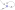
\includegraphics[width=100px]{fig3.pdf}
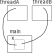
\includegraphics[width=100px]{fig4.pdf} \\\\
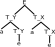
\includegraphics[width=200px]{fig5.pdf} \\\\

\includegraphics[width=200px]{fig6.pdf}



\fiche{Méthodes d'exclusion mutuelle}
\titre{Solution matérielle :} Le processus indique au CPU d'ignorer les interruptions. 
	\begin{itemize}
		\item Avantage : Plus de préemption imposée
		\item Inconvénients : Cette méthode est très dangereuse, elle compromet tout le système et exige de stopper tous les CPU.
	\end{itemize}

\titre{Solution logicielle 1 : L'alternance stricte} Variable "verrou" et attente active. Attention : "Test and Modify" ne marche pas. \\
\begin{minipage}{0.5\linewidth}
Algo A : \\
\\
Tantque vrai faire\\
  //section non critique\\
	Tantque verrou != 0 faire \\
		rien \\
	Fin Tantque\\
	verrou $\leftarrow$ 1\\
Fin Tantque\\
\end{minipage}
\begin{minipage}{0.5\linewidth}
Algo B : \\
\\
Tantque vrai faire\\
  //section non critique\\
	Tantque verrou != 1 faire \\
		rien \\
	Fin Tantque\\
	verrou $\leftarrow$ 0\\
Fin Tantque\\
\end{minipage}

\begin{itemize}
	\item Avantage : Simple, purement logiciel
	\item Inconvénient : Alternance stricte (pb résolu par Peterson), forte consommation CPU
\end{itemize}

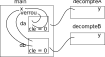
\includegraphics[width=200px]{fig7.pdf}

\\
\titre{Problème producteur / consommateur : } On a $n$ processus ou threads qui produisent des données. Ces données sont traitées par $m$ autres processus ou threads. (souvent $n > 1$ et $m = 1$. Exemple : le spool d'impression). \\
Solution naïve :
\begin{itemize}
	\item Données : 
	\begin{itemize}
		\item un tableau Tab de taille $N$. (dans lequel les producteurs écrivent et les consommateurs lisent)
		\item un entier lib représentant l'indice de la première case libre pour écrire
		\item un entier occ représentant l'indice de la première case occupée pour lire
		\item un entier nbocc indiquant le nombre de cases occupées.
		\item un entier nblib indiquant le nombre de cases libres.
	\end{itemize}
	\item Initialisation :
	\begin{itemize}
		\item lib et occ valent 0, nb\_lib = N et nb\_occ = 0.
	\end{itemize}
	\item Producteur : \\
\\ 
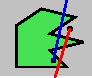
\includegraphics{fig12.pdf}
	\item Consommateur : \\
\\ 
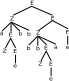
\includegraphics{fig13.pdf}
\end{itemize}

\titre{Sémaphore :} (Dijkstra 1965) Un entier muni de deux fonctions \titre{POST} et \titre{WAIT} et une file d'attente. La file d'attente contient des processus ou threads bloqués sur le sémaphore. \\
\begin{itemize}
	\item POST : \\
\\ 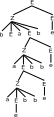
\includegraphics{fig14.pdf}
	\item WAIT : \\
\\ 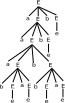
\includegraphics{fig15.pdf}
	\item Contrainte : Les fonctions POST et WAIT doivent être implémentées de manière à ne jamais être interrompues. On parle d'une solution matérielle ET logicielle.
	\item Lorsqu'un processus est bloqué il ne consomme aucun temps CPU
	\item Lorsque des processus sont bloqués sur le sémaphore, son entier vaut forcément 0 (la réciproque est fausse)
\end{itemize}

\titre{Solution à l'exclusion mutuelle :} \\
\\	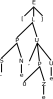
\includegraphics{fig16.pdf} \\
\titre{Solution du producteur / consommateur :}
\begin{itemize}
	\item Données : 
	\begin{itemize}
		\item un tableau Tab de taille $N$. (dans lequel les producteurs écrivent et les consommateurs lisent)
		\item un entier lib représentant l'indice de la première case libre pour écrire
		\item un entier occ représentant l'indice de la première case occupée pour lire
		\item un sémaphore nbocc qui compte les cases occupées
		\item un sémaphore nblib qui compte les cases libres
		\item un sémaphore excl pour gérer l'exclusion mutuelle
	\end{itemize}
	\item Producteur : \\
\\ 
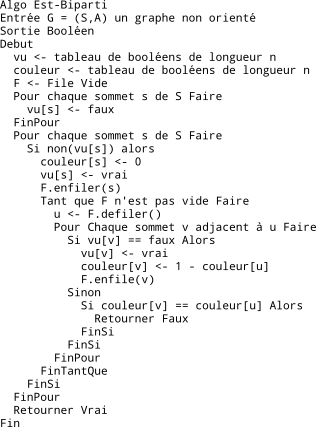
\includegraphics{fig17.pdf}
	\item Consommateur : \\
\\ 
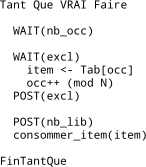
\includegraphics{fig18.pdf}
\end{itemize}

\titre{Mutex :} Sémaphore binaire servant uniquement à assurer l'exclusion mutuelle. L'entier est remplacé par deux états possibles : verrouillé ou déverrouillé. Les 2 fonctions s'appellent alors LOCK et UNLOCK \\

\titre{Sémaphore nommé / non nommé :} Un sémaphore nommé apparait dans le système de fichier (plusieurs processus qui ne se connaissent pas peuvent l'utiliser) (c'est un fichier virtuel, les droits d'accès s'appliquent).  Un sémaphore non nommé est simplement une variable de notre processus (partagée entre nos threads uniquement).



\fiche{TD1}
\titre{question 1} \\ Exemple basique de fork : une variable est dupliquée du père au fils. \\
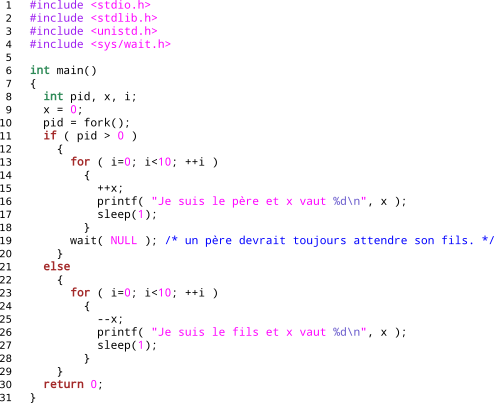
\includegraphics[width=\linewidth]{fig25.pdf}\newpage
\titre{question 2}
\begin{enumerate}
	\item Deux threads manipulent la même variable globale \\
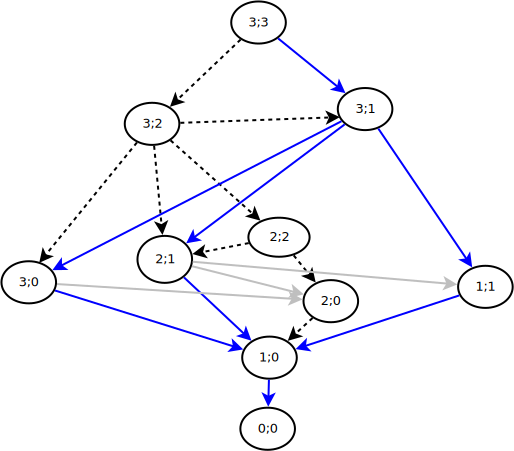
\includegraphics[width=\linewidth]{fig26.pdf}\newpage
	\item Deux threads manipulent la même variable grâce aux pointeurs \\
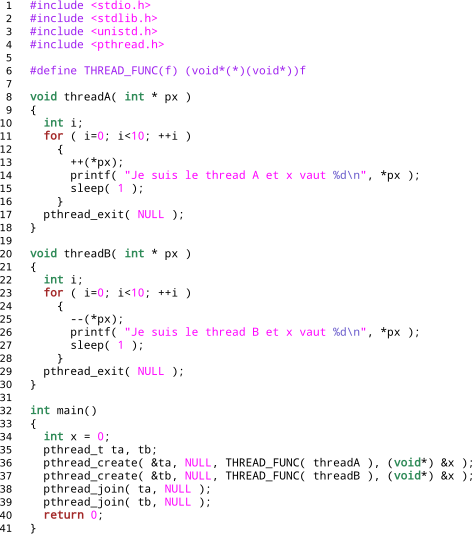
\includegraphics[width=\linewidth]{fig27.pdf}\\
\end{enumerate} \newpage
\titre{question 3}
\begin{enumerate}
	\item Deux threads décrémentent un même variable\\
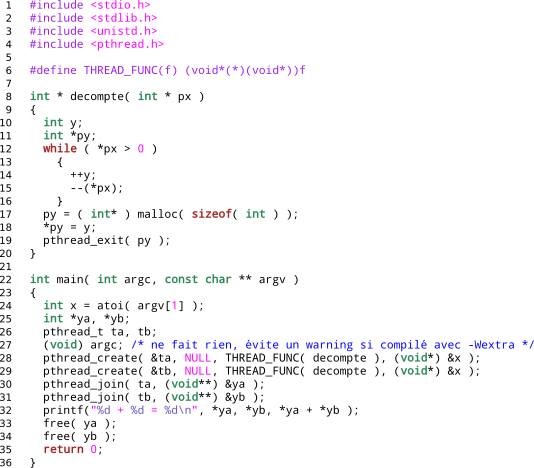
\includegraphics[width=\linewidth]{fig28.pdf}\newpage
	\item Nous essayons d'utiliser un verrou pour éviter les problèmes de concurrence (attente active)\\
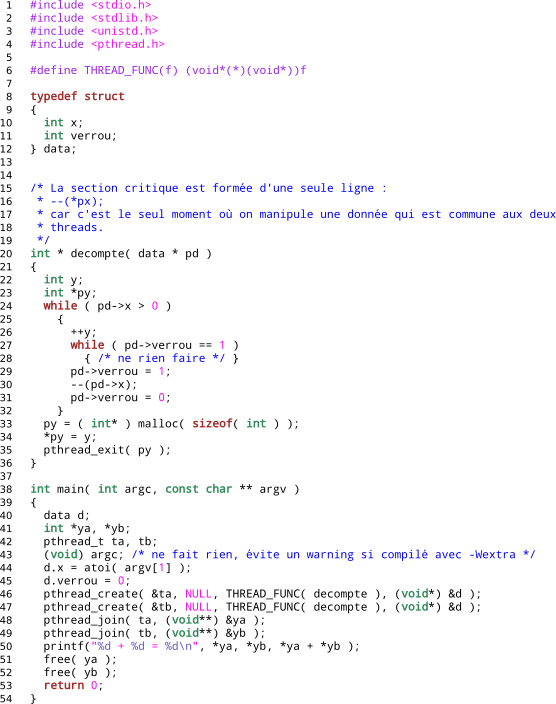
\includegraphics[width=\linewidth]{fig29.pdf}\\
\end{enumerate}


\fiche{TD2}
\titre{Exercice 1 :}
\begin{enumerate}
	\item Condition de concurrence : le résultat final dépend de l'ordonnancement
	\item Section critique : portion de code où deux processus ne devraient jamais se trouver en même temps sous peine de créer une condition de concurrence.
\end{enumerate}

\titre{Exercice 2}
\begin{enumerate}
	\item La création d'un thread est plus rapide que la création d'un processus.
	\item Pour être le plus général possible. Pour plusieurs variables on crée une struct. (idée : créer une fonction bidon qui va répartir les champs de la struct en argument et appeler la fonction qu'on veut)
	\item Il sert à enregistrer le retour d'une fonction.
	\item La valeur renvoyée par pthread\_join et pthread\_create est 0 pour un succès, autre chose pour une erreur.
\end{enumerate}

\titre{Exercice 3}
\begin{enumerate}
	\item 1,5 secondes
	\item 15 + 100*75 = 7515
	\item 100*15 + 10*75 = 2250 \\ 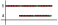
\includegraphics[width=200px]{fig8.pdf}
	\item 1,5 secondes \\ 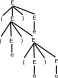
\includegraphics[width=200px]{fig9.pdf}
\end{enumerate}

\titre{Exercice 4}
\begin{enumerate}
	\item Un thread peut s'activer sur les requetes en cache pendant qu'un autre attend le disque dur
	\item L'appel à pthread\_create échouera si on dépasse le nombre maximal de thread autorisé
	\item  .\\ 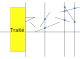
\includegraphics[width=300px]{fig10.pdf}

\end{enumerate}

\titre{Exercice 5 :} 
\begin{enumerate}
	\item $A1, A2, A3, A4, A5, B1, B2, B3, B4, B5, B6, B7, A6, A7$
	\item La section critique est composée des lignes 4 à 6
	\item Inverser les lignes 5 et 6 (la copie du document n'a pas besoin d'être en section critique.
\end{enumerate}

\titre{Exercice 6 :} \\
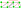
\includegraphics[width=300px]{fig11.pdf}


\fiche{TD3}
\input{2901.tex}

\fiche{Mémoire partagée}
\titre{Principe :} Avoir des pages de mémoire inscrites dans l'espace d'adressage de plusieurs processus.\\
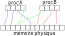
\includegraphics[width=200px]{fig19.pdf}

\titre{Avantage :} C'est le moyen le plus rapide d'échanger des données entre deux processus.\\

\titre{Inconvénient :} C'est aussi un très bon moyen pour créer des conditions de concurrence.\\

\titre{Comment ça marche ?} 
\begin{enumerate}
	\item Un processus crée un fichier virtuel (shm\_open)
	\item On redimensionne le fichier à la taille voulue (ftruncate)
	\item Projeter le fichier virtuel dans l'espace d'adressage du processus (mmap)
	\item Les processus qui veulent l'utiliser ouvrent le fichier (shm\_open) et le projettent dans leur espace d'adressage (mmap)
	\item Les processus utilisent cette mémoire partagée (attention aux conditions de concurrence)
	\item Lorsqu'un processus a terminé il ferme la projection (munmap) et le fichier (fclose)
	\item Lorsque tous les processus ont terminé, on détruit le fichier (shm\_unlink)
\end{enumerate}


\fiche{Exo Fork et mémoire partagée}
\titre{Exemple prof :}  Le processus mp1 crée un espace partagé de la taille d'un entier et demande en boucle à l'utilisateur de changer la valeur de cet entier. Le processus mp2 utilise cet espace partagé et affiche en boucle la valeur de l'entier toutes les secondes. \\

\titre{Modifications apportées pour tester ce qu'il se passe lors d'un fork :} Je n'ai pas modifié le fichier mp1. Par contre dans le fichier mp2 j'ai fait un fork avant d'entrer dans la boucle, puis dans la boucle, le processus indique s'il est le père ou le fils avant d'afficher la valeur de l'entier.\\

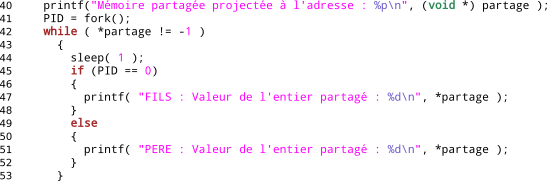
\includegraphics[width=\linewidth]{fig21.pdf}

\titre{Conclusion :} On pouvait naturellement imaginer que les deux processus allaient reconnaitre la valeur de l'entier partagé. En effet, la mémoire est copiée du père au fils, et l'espace mémoire mappé est donc copié avec son mapping, donc dans le fils le mapping vers le fichier virtuel existe toujours. C'est bien ce résultat attendu qui s'est produit. \\

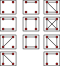
\includegraphics[width=\linewidth]{fig20.pdf}\\


\includegraphics[width=\linewidth]{fig22.pdf}


\fiche{Variables de condition}
\titre{Scénario classique :} \\
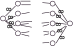
\includegraphics[width=300px]{fig32.pdf}\\

\titre{Utilisation :} Une \titre{Variable de condition} s'utilise toujours de paire avec un mutex. \\

\titre{3 primitives :}
\begin{enumerate}
	\item cond\_wait(C: Variable de condition, M:Mutex). Doit être appelé à l'intérieur d'une section critique protégée par M. Ce que ça fait :
	\begin{enumerate}	
		\item unlock(M)
		\item attendre un signal sur C
		\item lock(M)
	\end{enumerate}
	Intérêt de l'appel système pour faire ça : le passage de a à b est atomique, tout comme le passage entre b et c.
	\item cond\_signal(C: Variable de condition) Débloque au moins un processus bloqué sur C.
	\item cond\_broadcast(C: Variable de condition) Débloque tous les processus bloqués sur C.
\end{enumerate}

\titre{Remarque :} 
\begin{enumerate}
	\item Les variables de condition sont sans mémoire. Un signal émis lorsqu'aucun processus n'est en attente est perdu.
	\item Un cond\_wait s'exécute toujours à l'intérieur d'un tantque.
\end{enumerate} 

\includegraphics[width=300px]{fig33.pdf}\newpage

\titre{Producteurs/consommateurs :}\\
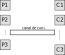
\includegraphics[width=200px]{fig34.pdf}\\


\fiche{Barrières de synchronisation}
\titre{Outils de synchronisation :}
\begin{itemize}
	\item Sémaphore
	\item Mutex
	\item Variables de condition 
	\item Barrières
	\item Tubes
\end{itemize}

\titre{Principe des barrières :} Une barrière sert à bloquer des processus et à les débloquer lorsqu'un certain nombre ont atteint la barrière. \\

\titre{Une seule primitive :} barrier\_wait(B:Barriere) bloque le thread jusqu'à ce qu'un nombre suffisant d'appels à barrier\_wait aient été effectués. 


\fiche{Tubes}
\titre{Descripteurs de fichier :} Il s'agit d'un nombre entier utilisé ppour identifier un fichier ouvert par un processus. L'OS maintient pour chaque processus une table des descripteurs. \\
Par défaut, 3 descripteurs sont associés à notre programme\\
\begin{tabular}{l|l}
Descripteur & fichier \\ \hline
0 & stdin : lecture du clavier \\ \hline
1 & stdout : écriture dans le terminal \\ \hline
2 & stderr : écriture dans le terminal \\ \hline
\end{tabular} \\
Puis lorsque l'utilisateur réalise la commande open, un nouveau descripteur est créé.\\

\titre{Manipulation :}
\begin{enumerate}
	\item Lecture : read(int fd, void* buf, size\_t count). fd est le descripteur, buf est l'espace mémoire où l'OS va écrire les données lues, et count le nombre d'octets à lire. Retourne le nombre d'octets qui ont réellement été lus, et -1 si erreur.
	\item Ecriture : write(int fd,const void* buf, size\_t count). fd est le descripteur, buf est l'espace mémoire où l'OS va lire les données à écrire dans le fichier, et count le nombre d'octets à écrire. Retourne le nombre d'octets qui ont réellement été écrits, et -1 si erreur.
\end{enumerate}

\titre{Tube : } Fichier virtuel implémentant un canal de communication unidirectionnel. Il a deux extrémités : une en lecture et une en écriture. On manipule les tubes à l'aide de descripteurs de fichiers associés aux extrémités.\\

\titre{Fonctionnement : } 
\begin{enumerate}
	\item Un read effectué sur un tube vide bloque le thread appelant jusqu'à ce qu'un autre thread y écrive des données
	\item Un write effectué sur un tube plein bloque le thread appelant jusqu'à ce qu'un autre thread y lise les données, libérant ainsi de l'espace. 
	\item L'OS garantit que read et write sont atomiques sur les tubes, à condition que la taille des données ne dépasse pas la taille du tube (constante PIPE\_BUF définie dans limits.h) . 
	\item Pour lire ou écrire dans un tube, il faut que les deux extrémités aient été ouvertes. Un tube dont une des extrémités est fermée est dit cassé. 
	\begin{enumerate}
		\item Ecrire dans un tube cassé provoque une erreur
		\item Lire dans un tube vide et cassé ne lit rein et retourne 0.
	\end{enumerate}
\end{enumerate}

\titre{Nommés / non nommés :} Un tube nommé apparait dans le système de fichier, contrairement au non nommé. \\
	\begin{enumerate}
		\item Création de Non nommés :
		\begin{enumerate}
			\item Dans le terminal en séparant deux programmes par le symbole pipe | 
			\item Par la commande int pipe(int df[2]) (df[0] = descripteur du fichier en lecture, df[1] = descripteur du fichier en écriture)
		\end{enumerate}
		\item Création d'un tube nommé
		\begin{enumerate}
			\item mkfifo nomFichier
		\end{enumerate}
	\end{enumerate}
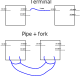
\includegraphics[width=200px]{fig35.pdf} \\
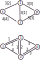
\includegraphics[width=180px]{fig36.pdf} \\


\fiche{Problèmes liés à la synchronisation}
\titre{Resource :} Objet physique ou virtuel pouvant être alloué à un seul processus à la fois.\\

\titre{Resources retirables :} Peut être retirée au processus, utilisé par un autre, puis rendu au premier sans compromettre son exécution (exemples : CPU, RAM). \\

\titre{Resources non retirables :} Ne peut être retirée au processus que lorsqu'il en aura décidé. \\

\titre{3 étapes pour accéder à une resource non retirable :}
\begin{enumerate}
	\item Solliciter la resource
	\item Utiliser la resource
	\item Libérer la resource
\end{enumerate}

\titre{Famine :} Situation où un processus demande l'accès à une ressource mais ne l'obtient jamais car elle est toujours attribuée à d'autres processus.\\

\titre{Solution :} Le principe FIFO permet d'éviter la famine mais n'est pas toujours souhaitable. \\

\titre{Interblocage :} Situation où un ensemble de processus attendent un événement que seul un des processus de l'ensemble peut provoquer.\\

\titre{Exemple :}\\
\begin{tabular}{l|l}
Proc A & Proc B \\ \hline
Lock(M1) & Lock(M2) \\ 
Lock(M2) & Lock(M1) \\
\ldots & \ldots \\
Unlock(M2) & Unlock(M1) \\
Unlock(M1) & Unlock(M2) \\
\end{tabular}

\titre{Modélisation du problème : Modèle de Holt } (1972) On trace le graphe des attentes qui contient deux types de sommets (carré = ressource, rond = processus) \\
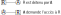
\includegraphics[width=100px]{fig37.pdf}\\

\titre{Exemple :}\\
\begin{tabular}{l|l|l}
A & B & C \\ \hline
D(R) & D(S) & D(T) \\
D(S) & D(T) & D(R) \\
L(R) & L(S) & L(T) \\
L(S) & L(T) & L(R) \\
\end{tabular} \\
Si l'ordonnancement est A,B,C,A,C on obtient : \\
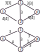
\includegraphics[width=100px]{fig38.pdf} \\

\titre{Stratégie face aux interblocages}
\begin{enumerate}
	\item Les ignorer
	\item Les détecter et y remédier 
	\begin{itemize}
		\item Mettre à jour dynamiquement le graphe des attentes lancer périodiquement un algo de détection des cycles. En cas d'interblocage on tue un des processus et on libère toutes ses ressources.
	\end{itemize}
	\item Détecter dynamiquement si il est sûr d'allouer une ressource
	\begin{itemize}
		\item 
		\begin{tabular}{l|l}
			A & B \\ \hline
			D(R) & D(S) \\
			D(S) & D(R) \\
			L(R) & L(S) \\
			L(S) & L(R) \\
		\end{tabular} \\
		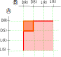
\includegraphics[width=100px]{fig39.pdf} \\
		On appelle état sûr un état à partir duquel on peut exécuter tous les processus un après l'autre dans un certain ordre sans qu'aucun ne soit bloqué. Un interblocage survient toujours à partir d'un état non sûr. \\ Pour déterminer les états sûrs, il faut connaitre à l'avance le code que vont exécuter les programmes. 
	\end{itemize}
	\item Imposer des contraintes pour s'assurer qu'un interblocage est impossible
	\begin{itemize}
		\item Pas d'exclusion mutuelle
		\item Ordonne les ressources
	\end{itemize}
\end{enumerate}


\end{document}
